
\documentclass[12pt]{article}
\usepackage{graphicx}
\usepackage{amsmath}
\usepackage{mathtools}
\usepackage{gensymb}
\usepackage{tabularx}
\usepackage{array}
\usepackage[latin1]{inputenc}
\usepackage{fullpage}
\usepackage{color}
\usepackage{array}
\usepackage{longtable}
\usepackage{calc}
\usepackage{multirow}
\usepackage{hhline}
\usepackage{ifthen}
\usepackage{lscape}
\usepackage{float}
\usepackage{amssymb}

\newcommand{\mydet}[1]{\ensuremath{\begin{vmatrix}#1\end{vmatrix}}}
\providecommand{\brak}[1]{\ensuremath{\left(#1\right)}}
\providecommand{\cbrak}[1]{\ensuremath{\left\{#1\right\}}}
\providecommand{\norm}[1]{\left\lVert#1\right\rVert}
\providecommand{\abs}[1]{\left\vert#1\right\vert}
\newcommand{\solution}{\noindent \textbf{Solution: }}
\newcommand{\myvec}[1]{\ensuremath{\begin{pmatrix}#1\end{pmatrix}}}
\let\vec\mathbf

\def\inputGnumericTable{}

\begin{document}
\begin{center}
\textbf\large{OPTIMIZATION}

\end{center}
\section*{Excercise 10.3}

Q.3.2 Reduce the equation $y-2=0$ into normal form. Find the perpendicular distances from the origin and angle between perpendicular and the positive x-axis.

\solution
The given equation can be written as
\begin{align}
	\label{eq:eq1}
	\myvec{0&1}\vec{x} &= 2
\end{align}
Let $\vec{O}$ be the point from where we have to find the perpendicular distance. The perpendicular distance will be the minimum distance from $\vec{O}$ to theline. Let $\vec{P}$ be the foot of perpendicular. This can be formulated as an optimization problem as follows:
\begin{align}
	\min_{\vec{x}}f\brak{\vec{x}} &= \norm{\vec{x}-\vec{O}}^2\\
	\text{s.t. } g\brak{\vec{x}} &= \vec{n}^\top\vec{x}-c=0
\end{align}
where
\begin{align}
	\vec{n} &= \myvec{0\\1}\\
	\vec{O} &= \myvec{0\\0}\\
	c &= 2
\end{align}
Now we define
\begin{align}
	H\brak{\vec{x},\lambda} = f\brak{\vec{x}} - \lambda g\brak{\vec{x}}
\end{align}
and we find that
\begin{align}
	\nabla f\brak{\vec{x}} &= 2\brak{\vec{x}-\vec{O}}\\
	\nabla g\brak{\vec{x}} &= \vec{n}
\end{align}
We have to find $\lambda \in \mathbb{R}$ such that
\begin{align}
	\nabla H\brak{\vec{x},\lambda} &= 0\\
	\label{eq:eq2}
	\implies 2\brak{\vec{x}-\vec{O}}-\lambda\vec{n} &= 0\\
	\label{eq:eq3}
	\implies \vec{x} = \frac{\lambda}{2}\vec{n}+\vec{O}
\end{align}
Substituting \eqref{eq:eq3} in \eqref{eq:eq1}
\begin{align}
	\vec{n}^\top\brak{\frac{\lambda}{2}\vec{n}+\vec{O}} - c &= 0\\
	\implies \lambda &= \frac{2\brak{c-\vec{n}^\top\vec{O}}}{\norm{\vec{n}}^2}
\end{align}
Substituting the value of $\lambda$ in \eqref{eq:eq3},
\begin{align}
	\vec{x}_{min} &= \vec{P} = \vec{O}+\frac{\vec{n}\brak{c-\vec{n}^\top\vec{O}}}{\norm{\vec{n}}^2}\\
	&= \myvec{0\\0}+ \frac{\myvec{0\\1}\brak{2-\myvec{0&1}\myvec{0\\0}}}{1}\\
	&= \myvec{0\\0}+\myvec{0\\2}\\
	&= \myvec{0\\2}\\
	OP &= \norm{\vec{P}-\vec{O}}^2\\
	&= \sqrt{0^2+2^2} = 2
\end{align}
The angle $\theta$ made by this perpendicular with x-axis is given by
\begin{align}
	\theta &= \tan^{-1}{\brak{\frac{2}{0}}}\\
	&= 90\degree
\end{align}
The normal form of equation for straight line is given by 
\begin{align}
	\myvec{\cos{90}\degree&\sin{90}\degree}\vec{x} = 0
\end{align}
See figure \ref{fig:Fig1}
\begin{figure}[!h]
	\begin{center} 
	    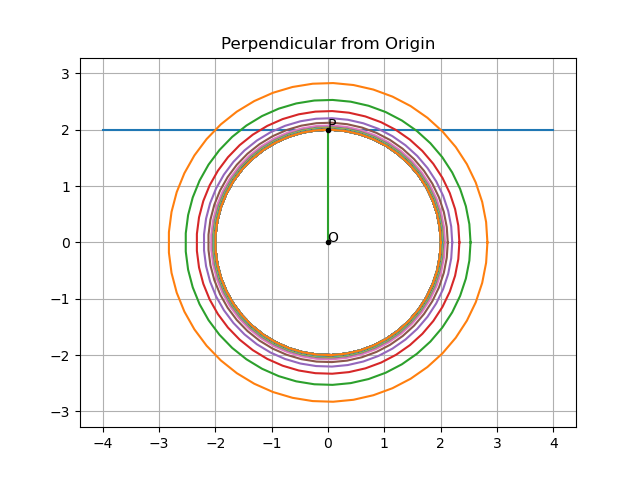
\includegraphics[width=\columnwidth]{figs/opt3}
	\end{center}
\caption{}
\label{fig:Fig1}
\end{figure}

\end{document}




























